\documentclass[10pt]{article}
\usepackage[margin=0.58in]{geometry}
\usepackage[T1]{fontenc}
\usepackage{lmodern}
\usepackage{graphicx}
\usepackage{booktabs}
\usepackage[colorlinks=true,urlcolor=blue]{hyperref}
\pagestyle{empty}
\begin{document}
\begin{center}
{\Large APS native export and bounded audit reader}\\[3pt]
2026-11-04 --- component development report
\end{center}
\noindent
The Rust adapter constructs the canonical experiment export from a pinned
protocol, saved plan, literal record lines and explicit execution-history
sidecar. The reader uses separate ordinary-residue affine arithmetic and
source reconstruction. All development assertions here have producer standing
\texttt{[pcc:unverified]}; no signed execution result is supplied.

\begin{center}
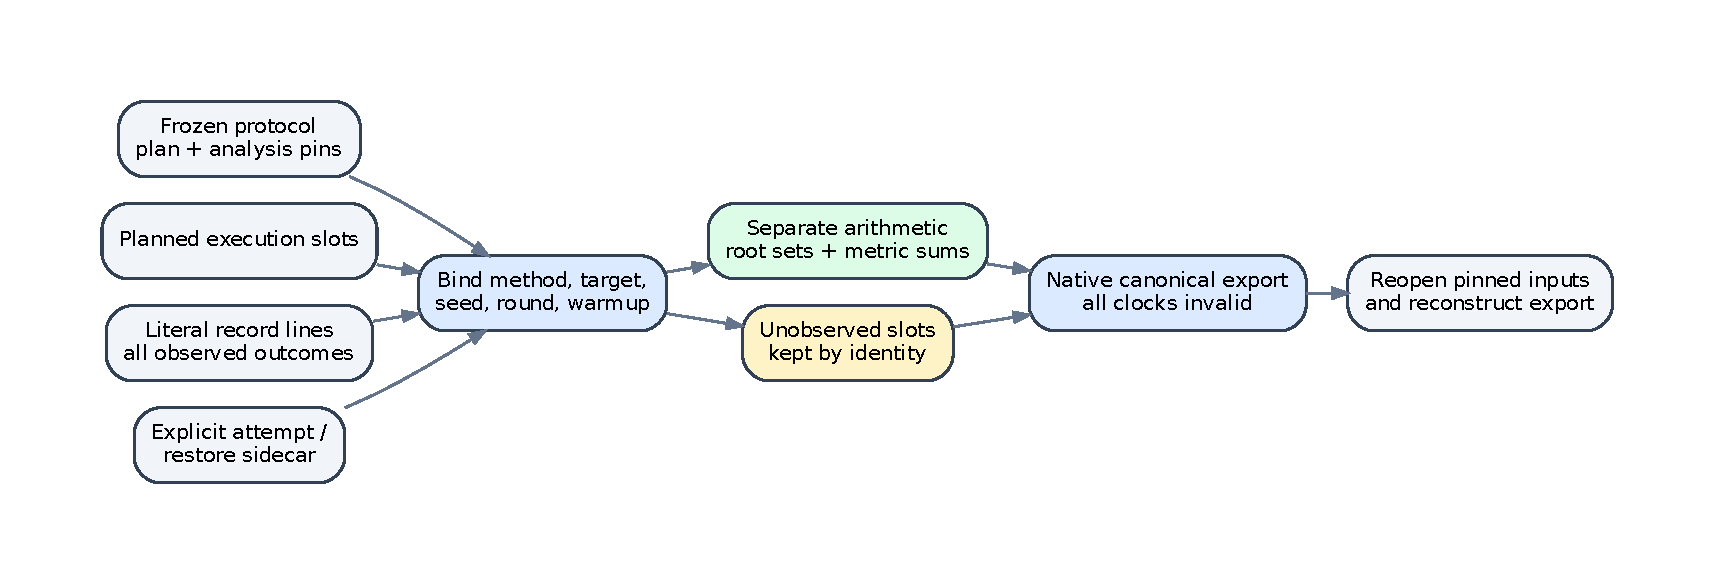
\includegraphics[width=\linewidth]{pipeline.pdf}
\end{center}
\noindent\textbf{Collection and consistency.}
Rows retain failures, late witnesses and recordless infrastructure outcomes.
Every unobserved planned slot remains visible by identity, without an invented
attempt or exclusion. Checking reconstructs the complete export from pinned
input bytes; an incomplete observed population cannot pass the complete check.

\medskip
\noindent\textbf{Bounded mathematical and metric reader.}
The explicit-curve guard covers prime fields up to 65,521. Checks include
subgroup membership, labeled points, signed coefficients, nonzero denominator
and recovered scalar; cubic pruning additionally requires the map/eigenvalue
and propagated labels. A direct point oracle compares attempts claiming complete
root sets, capped at one million sign candidates per record. Partial root
sets remain partial. Six cold phases and five online phases are recomputed,
along with the producer's retained partial diagnostics.

\begin{center}
\begin{tabular}{lr}
\toprule
Producer-reported development checks & Outcome\\
\midrule
Standalone release library & 42 passed, 0 failed\\
Native command-line pipeline & 5 passed, 0 failed\\
Strict Clippy: Rust 1.98 and stable & exit 0 each\\
Workflow syntax & exit 0\\
Actual producer bridge & 3 passed, 0 failed\\
Broad repository library & running; failures observed\\
\bottomrule
\end{tabular}
\end{center}
\noindent
Claim \texttt{PCC-20261104-56667f}: unverified. Normalized commands, source
pins and original-log digests are in \path{validation/source-freeze-summary.json}.
The first draft's invalid one-arm fixture and the bridge's corrected crate-name
import are retained as development failures. These counts are not timings or
experimental samples. Final protocol fixtures are wholly synthetic; copied
historical runtime metadata was rejected for publication and replaced.
\href{https://github.com/isogeny-labs/crypto/tree/a6630cd83e25ca5eed3d88d64503f12b30402094}{Source commit \texttt{a6630cd83e25}} pins the component.

\medskip
\noindent\textbf{Explicit boundaries.}
Packaging does not qualify a clock or attest execution, sampler history,
complete native work, polynomial-construction fidelity or full curve order.
All exported clocks remain invalid. Next steps are complete operation pricing,
the held-out four-size protocol/analysis and external comparison, followed by
maintained run admission. The approved source checkpoint awaits configured
authentication. No performance session or benchmark row is reported.
Publication of the companion native ledger is blocked pending explicit
approval; merging remains disabled.

\medskip
\noindent\textbf{Sources.}
APS revised manuscript \S\S3.1--3.4; prior APS four-lead and replay contracts;
canonical \texttt{experiment.protocol/v1} and \texttt{experiment.export/v1} at
crypto-autoresearcher \texttt{774611edb0a5}; the native pencil exporter's
study-specific reconstruction contract; repository PCC and measurement rules.
\end{document}
